\section{RESULTS}
\begin{frame}{\secname}
\end{frame}

\subsection{Model performances}
\begin{frame}{\subsecname}
After tuning, the models can be ranked as follows:

\begin{table}
    \centering
    \begin{tabular}{l|cc}
         & Class 1 recall & Recall macro average \\
         \hline\hline
         \textbf{Random Forest} & 84\% & \textbf{89\%} \\
         \textbf{SVM} & \textbf{85\%} & 88\% \\
         SGD & 80\% & 80\% \\
         Perceptron & 72\% & 79\% \\
         Decision Tree & 71\% & 83\% \\
         AdaBoost & 55\% & 77\% \\
         KNN & 45\% & 72\% \\
         Gaussian NB & 34\% & 66\% \\
    \end{tabular}
    \label{tab:my_label}
\end{table}

We therefore see that the Random Forest and SVM models can both be considered the most performant. However, being a few orders of magnitude faster to train, the former may be considered more optimal.

\end{frame}

\begin{frame}{\subsecname}
\begin{figure}
    \centering
    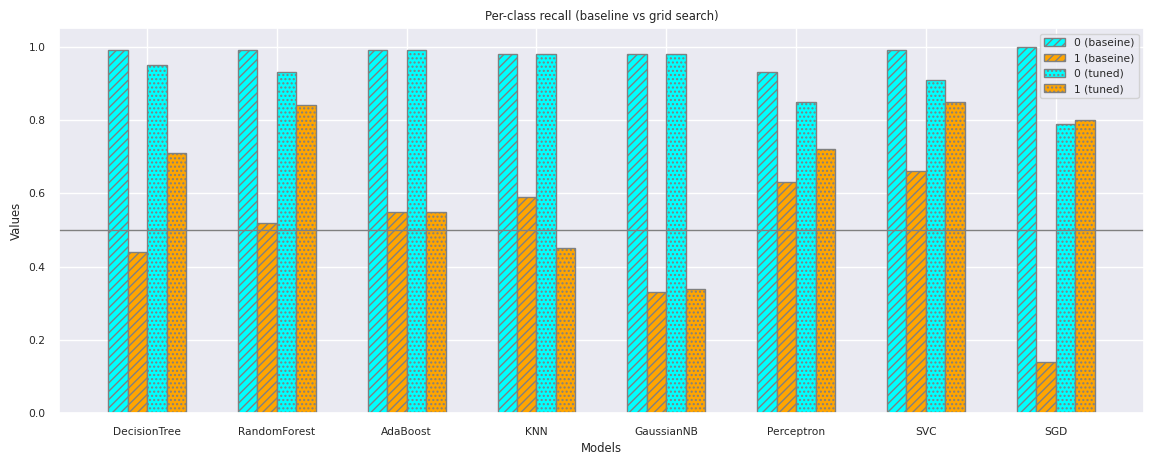
\includegraphics[width=1\linewidth]{images/recalls_before_after.png}
    \caption{Class recall before and after tuning}
    \label{fig:recall_before_after}
\end{figure}
\end{frame}

\begin{frame}{\subsecname}
\begin{figure}
    \centering
    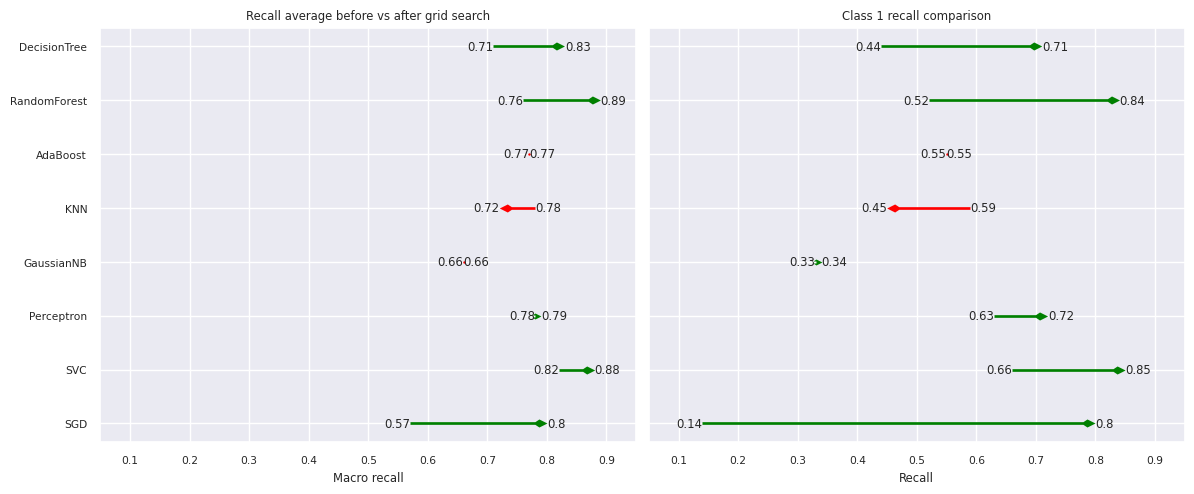
\includegraphics[width=1\linewidth]{images/recall_change.png}
    \caption{Class 1 recall and \txt{recall_macro} change with tuning}
    \label{fig:recall_change}
\end{figure}
\end{frame}

\subsection{Conclusions}
\begin{frame}{\subsecname}
The particularly bad performance of the KNN and Gaussian Naive Bayes classifiers was, to be fair, expected, though for different reasons:
\begin{itemize}
    \small
    \justifying
    \item For the former, the plots in figure \ref{fig:pairplots} show that the two classes are mostly overlapping and to not form well distinct clusters
    \item For the latter, its basic assumption of conditional independence between the attributes is clearly faulty in this context, since (for example) the rotational speed of a machine obviously influences its operating temperature
\end{itemize}

Furthermore, figure \ref{fig:recall_change} shows that these two models, and AdaBoost, either didn't improve or became worse. This may have two reasons:
\begin{itemize}
    \small
    \justifying
    \item none have a "class weight" parameter, and thus couldn't be tuned to "pay more attention" to one class than the other
    \item cross-validation is performed on a \textit{slice} of the training set (unlike the default model, which used all of it). This is especially damning for the KNN classifier because it doesn't really perform any analysis of the training data, instead simply using it "as-is".
\end{itemize}

\end{frame}

\begin{frame}{\subsecname}
The main focus of this project ended up being \textit{how to deal with severely imbalanced data}, more than a classification task itself. This, at least for the given dataset, was achieved in three main ways:
\begin{enumerate}
    \justifying
    \small
    \item using a per-class weighing of the datapoints, when supported
    \item performing dataset resampling during preprocessing to make the minority class easier to learn
    \item targeting the \txt{recall_macro} scoring metric when tuning instead of accuracy or precision
    \begin{itemize}
        \item this metric is an \textit{unweighted} average of the recalls for each class, making thus sure that the result doesn't de-facto only account for the majority datapoints
        \item the majority class being so dominant, it is acceptable to be slightly less accurate in classifying it if it means being way more sensitive to the minority
    \end{itemize}
\end{enumerate}

\end{frame}